\newpage
\section{LECTURE 5}

\section{Agenda}
In this lecture, we cover regularization, and line searches with constraints. We'll then move on to deterministic optimal control. 

\section{Regularization and Duality}
Consider the following problem: 
\begin{align}
    \min_x f(x) \\
    \ni c(x) = 0
\end{align}
We can express this as: 
\begin{align}
    \min_x f(x) + P_{\infty} (c(x)) \\
    P_{\infty} (x) = \begin{cases}
0, & x=0 \\
+ \infty, & x \neq 0 
\end{cases}
\end{align}
Practically, this is terrible, but we can get the same effect by solving:
\begin{align}
    \min_x \max_{\lambda} f(x) + \lambda^T c(x) 
\end{align}

\noindent
Whenever $c(x) \neq 0$, the inner problem gives $+\infty$. 
Similarly for inequalities: 
\begin{align}
    \min_x \ &f(x) \\
    \ni \ &c(x) \geq 0 \\
    &\implies \\
    \min_x \ &f(x) + P_{\infty}^+ (c(x))
\end{align}

\noindent
Here, we have: 
\begin{align}
    P_{\infty}^+ (x) &= \begin{cases}
0, & x \geq 0 \\
+ \infty, & x < 0 
\end{cases}
\implies \\ 
\min_x \max_{\lambda \geq 0} f(x) - \lambda c(x) 
\end{align}
where $f(x) - \lambda c(x)$ is our Lagrangian $L(x,\lambda)$.\\

\noindent
For convex problems, one can switch the order of the $\min$ and $\max$, and the solution does not change; this is the notion of ``dual problems''! This isn't true in general, however, i.e. for non-convex problems. \\

\noindent
The interpretation of this is that the KKT conditions define a saddle point in the space of $(x, \lambda)$. \\

\noindent
The KKT system should have $\dim(x)$ positive eigenvalues and $\dim(\lambda)$ negative eigenvalues at an optimum. Such a system is known as a ``Quasi-definite'' linear system. \\

\subsection{Take-Away Messages:}
\noindent
When regularizing a KKT system, the lower-right block should be negative! 
\begin{align}
    \begin{bmatrix}
        H + \alpha I \ \ \ \ C^T \\
        C \ \ \ \ -\alpha I 
    \end{bmatrix}
    \begin{bmatrix}
        \Delta x \\
        \Delta \lambda
    \end{bmatrix}
    = 
    \begin{bmatrix}
        -\nabla_x L \\
        - c(x)
    \end{bmatrix}
    , 
    \alpha > 0
\end{align}
This makes the system a quasi-definite one.

\noindent
Remember to check out the example of this in the lecture video. We observe that we still overshoot the solution, so we need a line search! 

\subsection{Merit Functions}
How do we a do a line search on a root-finding problem? Consider: 
\begin{align}
    \textrm{find} x* \ \ni \ c(x*) = 0
\end{align}
First, we define  a scalar ``merit function'' $P(x)$, that measure distance from a solution. 
A few standard choices for this merit function include: 
\begin{align}
    P(x) &= \frac{1}{2} c(x)^T c(x) = \frac{1}{2} || c(x) ||_{2}^2 \\
    \textrm{or} \ \ P(x) &= || c(x) ||_{1} \ \ \ \textrm{Note: Could use any norm}.
\end{align}
Now we could just do Armijo on $P(x)$: 
\\
\\
\noindent
\begin{algorithm}
	\caption{Armijo Rule on $P(x)$}
	\label{alg:armijo2}
	\begin{algorithmic}[1]	
        \State $\alpha = 1$  \Comment{Step Length}
        \While {$f(x + \alpha \Delta x) > f(x) + b \alpha \nabla f(x) ^T \Delta x$} \\ \Comment{$\alpha \nabla f(x) ^T \Delta x$ is the expected reduction from gradient, and $b$ is the tolerance.}
            \State $\alpha \gets c \alpha$ \Comment{$c$ is a scalar $<1$.}
        \EndWhile
        \State $x \gets \alpha \Delta x$
	\end{algorithmic}
\end{algorithm}
\\

\subsection{Constrained Minimization}
\noindent
How about constrained minimization? Here, we want to come up with an option that specifies how much we are violating the constraint, as well as how far off the optimum we are / minimizing the objective funciton. Consider the problem:
\begin{align}
    \min_x &f(x) \\
    \ni \ \ &c(x) \geq 0 \\
    \ni \ \ &d(x) = 0 \\
    \ &\ \implies \\
    L(x, \lambda, \mu) &= f(x) - \lambda^T c(x) + \mu^T d(x)
\end{align} \\

\noindent
We have lots of options for merit functions. One option is: 
\begin{align}
    P(x, \lambda, \mu) &= \frac{1}{2} || \nabla L(x, \lambda, \mu) ||_2^2 \\
\end{align}
Here, the term $\nabla L(x, \lambda, \mu)$ is the KKT residual: 
\begin{align}
    \begin{bmatrix}
        \nabla_x L(x,\lambda,\mu) \\
        \min(0, c(x)) \\
        d(x)
    \end{bmatrix}
\end{align}\\
However, this isn't the best option to use, because evaluating the gradient of the KKT condition is as expensive as the newton step solve itself.

\noindent
Another option is:
\begin{align}
    P(x,\lambda, \mu) &= f(x) + \rho \ || \begin{bmatrix}
        \min (0,c(x)) \\ 
        d(x) 
    \end{bmatrix} ||_1
\end{align}
Here, $\rho$ is a scalar trade off between the objective minimization and constraint satisfaction. Also remember that any norm works here (in place of the $1$ norm depicted), but using the $1$  norm is the most common. 
This option gives us flexibility, because we can pick trade off $\rho$ - initially we can set this to be low, to drive us close to the optimum solution, and when we are close to the optimum, we can increase $\rho$ to ensure we satisfy the constraints. 

Yet another option is: 
\begin{align}
    P(x, \lambda, \mu) &= f(x) - \Tilde{\lambda}^T c(x) + \Tilde{\mu}^T d(x) + \frac{\rho}{2} || \min(0,c(x) ||_2^2 + \frac{\rho}{2} || d(x) ||_2^2 
\end{align}
which is the augmented Lagrangian itself.

\noindent
Remember to check out the example in the lecture video! 

\subsection{Take-Away Messages (from the example)}
\begin{itemize}
    \item $P(x)$ based on the KKT residual is expensive. 
    \item Excessively large penalty weights can cause problems. 
    \item Augmented Lagrangian methods come with a merit function for free. So if we're using the Augmented Lagrangian to solve the problem, just use this as a merit function.
\end{itemize}

\\

\subsection{Deterministic Optimal Control}
Let's consider the following control problem:
\begin{align}
    \min_{x(t), u(t)} &= J(x(t), u(t)) = \int_{t_0}^{t_f} L(x(t), u(t)) dt + L_{F} (x(t_f)) \\
    \ni \ &\dot{x}(t) = f(x(t), u(t)) \\
    \ni \ &\textrm{Any other constraints} 
\end{align}
Here, we minimize across ``state'' or ``input'' trajectories. $J$ represents our cost function, $L(x(t), u(t))$ represents our ``stage cost'', $L_{F} (x(t_f))$ represents a ``terminal cost'', $\dot{x}(t) = f(x(t), u(t))$ are the dynamics constraint. \\

\noindent
This is an ``infinite dimensional'' problem in the sense that an infinite amount of discrete time control points required to fully specify the control to be applied. 
\begin{figure}[h!]
    \centering
    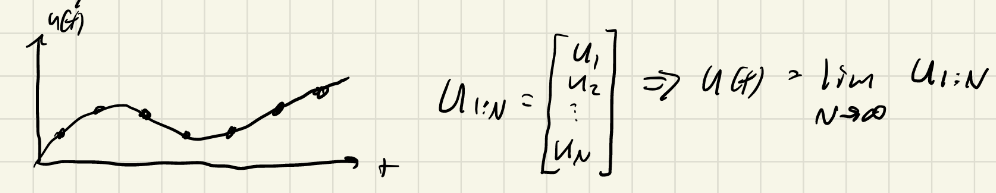
\includegraphics[width=0.4\linewidth]{L5_Images/L51.PNG}
    \caption{Deterministic optimal control problem}
    \label{fig:l5f1}
\end{figure}
\begin{itemize}
    \item The solutions to this problem are open loop trajectories. 
    \item Now, there are a few control problems with analytic solutions in continuous time, but not many. 
    \item We focus on the discrete-time setting, where we have tractable algorithms.
\end{itemize}

\subsection{Discrete Time}
Consider a discrete-time version of this problem. 
\begin{align}
    \min_{x_{1:N}, u_{1:N-1}} \ & J(x_{1:N}, u_{1:N-1}) = \sum_{k=1}^{N-1} L(x_k, u_k) + L_F(x_N) \\
    \ni \ & x_{n+1} = f(x_n,u_n) \\
    \ni \ & u_{\min} \leq u_k \leq u_{\max} \ \ \textrm{Torque limits.} \\
    \ni \ & c(x_k) \leq 0 \ \forall k \ \ \textrm{Obstacle / collision constraints.}
\end{align}
\begin{itemize}
    \item This version of the problem is now a finite dimensional problem.
    \item Samples $x_k,u_k$ are often called ``knot points''. 
    \item We can convert continuous systems to discrete-time problems using integration methods such as the Runge-Kutta method etc.
    \item Finally, we can convert back from discrete-time problems to continuous problems using interpolation. 
\end{itemize}
  


